\begin{figure}[htbp]
\centering
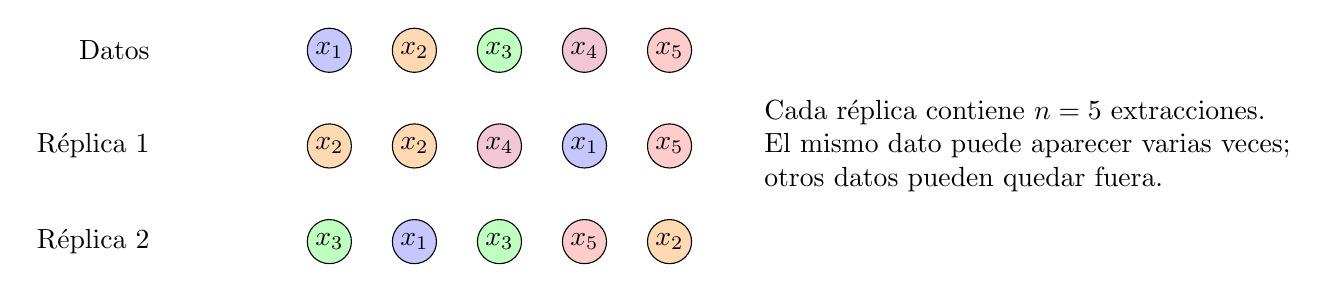
\begin{tikzpicture}[x=1.08cm,y=0.9cm,
  punto/.style={circle,draw,minimum size=0.56cm,inner sep=0pt},
  a/.style={punto,fill=blue!22}, b/.style={punto,fill=orange!30},
  c/.style={punto,fill=green!25}, d/.style={punto,fill=purple!22},
  e/.style={punto,fill=red!20}]
  \node[anchor=east] at (-1.0,0) {Datos};
  \foreach \i/\cl in {1/a,2/b,3/c,4/d,5/e}
    \node[\cl] at (\i,0) {$x_{\i}$};

  \node[anchor=east] at (-1.0,-1.35) {Réplica $1$};
  \foreach \j/\cl/\val in {1/b/2,2/b/2,3/d/4,4/a/1,5/e/5}
    \node[\cl] at (\j,-1.35) {$x_{\val}$};

  \node[anchor=east] at (-1.0,-2.7) {Réplica $2$};
  \foreach \j/\cl/\val in {1/c/3,2/a/1,3/c/3,4/e/5,5/b/2}
    \node[\cl] at (\j,-2.7) {$x_{\val}$};

  \node[anchor=west,align=left] at (6.0,-1.35)
    {Cada réplica contiene $n=5$ extracciones.\\El mismo dato puede aparecer varias veces;\\otros datos pueden quedar fuera.};
\end{tikzpicture}
\caption{Dos muestras bootstrap posibles extraídas con reemplazo de los cinco datos observados. El color identifica el dato de origen y permite ver las repeticiones.}
\label{fig:muestras-bootstrap}
\end{figure}